% !TEX TS-program = pdflatex
% !TEX encoding = UTF-8 Unicode

\documentclass[10pt,twocolumn]{article}

\usepackage{graphicx,listings,fixltx2e,lambda,array,times,fullpage}
\usepackage[usenames,dvipsnames]{xcolor}
\usepackage{color}

\definecolor{lightgray}{rgb}{0.92,0.92,0.92}

\lstset{ 
  language=Python,                % the language of the code
  linewidth=220pt, 
  xleftmargin=8pt,
  basicstyle=\footnotesize\ttfamily, % Standardschrift
  numbers=none,                   % where to put the line-numbers
  numberstyle=\footnotesize,          % the size of the fonts that are used for the line-numbers
  stepnumber=1,                   % the step between two line-numbers. If it's 1, each line 
                                  % will be numbered
  numbersep=5pt,                  % how far the line-numbers are from the code
  showspaces=false,               % show spaces adding particular underscores
  showstringspaces=false,         % underline spaces within strings
  showtabs=false,                 % show tabs within strings adding particular underscores
  frame=single,                   % adds a frame around the code
  tabsize=2,                      % sets default tabsize to 2 spaces
  captionpos=b,                   % sets the caption-position to bottom
  breaklines=true,                % sets automatic line breaking
  breakatwhitespace=false,        % sets if automatic breaks should only happen at whitespace
  title=\lstname,                   % show the filename of files included with \lstinputlisting;
                                  % also try caption instead of title
  numberstyle=\tiny\color{gray},        % line number style
  keywordstyle=\color{blue},          % keyword style
  commentstyle=\color{dkgreen},       % comment style
  backgroundcolor=\color{lightgray}, 
  belowskip=-10pt, 
  aboveskip=6pt, 
}


\begin{document}

\title{Parakeet: A Just-In-Time Parallel Accelerator for Python}
\author{
Alex Rubinsteyn \ \ \ \ Eric Hielscher \ \ \ \ Nathaniel Weinman \ \ \ \
Dennis Shasha \\
{\it Computer Science Department, New York University, New York, NY, 10003} \\
\small{\tt \{alexr,hielscher,nsw233,shasha\} @ cs.nyu.edu}
}
\date{}

% define some useful commands to use in language specification 
\newcommand{\MAP}{\impfnt{map}}
\newcommand{\REDUCE}{\impfnt{reduce}}
\newcommand{\SCAN}{\impfnt{scan}}
\newcommand{\ALLPAIRS}{\impfnt{allpairs}}
\newcommand{\concat}{\ensuremath{+\!\!\!\!+\,}}

\setlength\fboxsep{8pt}
\setlength\fboxrule{0.5pt}

\maketitle

\begin{abstract}
High level productivity languages such as Python or Matlab enable the use of computational resources by non-expert programmers.  However, these languages sacrifice program speed for ease of use, with this trade-off especially stark for modern parallel processors such as multicore CPUs and manycore GPUs.

In this paper, we discuss Parakeet, a library which provides a just-in-time (JIT) parallel accelerator for Python.  Parakeet bridges the gap between the usability of Python and the speed of code written in efficiency languages such as C++ or CUDA.  Parakeet accelerates data-parallel sections of Python that use the standard NumPy scientific computing library.  Parakeet JIT compiles efficient versions of Python functions and automatically manages their execution on both GPUs and CPUs.  We assess Parakeet on a pair of benchmarks and achieve significant speedups.  While Parakeet is a work in progress, our current results clearly demonstrate its promise.
\end{abstract}

\section{Introduction}
\label{Intro}
Numerical computing is an indispensable tool to professionals in a wide range of fields, from the natural sciences to the financial industry.  Often, users in these fields either (1) aren't expert programmers; or (2) don't have time to tune their software for performance.  These users typically prefer to use productivity languages such as Python or Matlab rather than efficiency languages such as C++.  Productivity languages facilitate non-expert programmers by trading off program speed for ease of use \cite{Pre03}.

A common problem, however, is that the performance tradeoff is often very stark -- code written in Python or Matlab~\cite{Moler80} often has much worse performance than code written in C++ or Fortran.  This problem is getting worse, as modern processors (multicore CPUs as well as GPUs) are all parallel, and current implementations of productivity languages are poorly suited for parallelism.  Thus a common workflow involves prototyping algorithms in a productivity language, followed by porting the performance-critical sections to a lower level language.  This second step can be time-consuming, error-prone, and it diverts energy from the real focus of these users' work.

In this paper, we present Parakeet, a library that provides a JIT parallel accelerator for NumPy, the commonly-used scientific computing library for Python~\cite{Oliphant07}. Parakeet accelerates performance-critical sections of numerical Python programs to be competitive with efficiency language code, obviating the need for the above-mentioned ``prototype, port'' cycle.

The Parakeet library intercepts programmer-marked functions and uses high-level operations on NumPy arrays (e.g.~mapping a function over the array's elements) as sources of parallelism. These functions are just-in-time compiled to either x86 machine code using LLVM~\cite{Latt02}, or GPU code that can be executed on NVIDIA GPUs via the CUDA framework~\cite{NvidCU}. These native versions of the functions are then automatically executed on the appropriate hardware. Parakeet allows complete interoperability with all of the standard Python tools and libraries.

Parakeet currently supports JIT compilation to parallel GPU programs and single-threaded CPU programs.  While Parakeet is a work in progress, our current results clearly demonstrate its promise.  In the near future, Parakeet's CPU support will be extended to use of multiple CPU cores.  We are also working on adding support for splitting computations across CPUs and GPUs simultaneously -- keeping all processors in a system busy at once -- and on-the-fly tuning of resource usage.

\section{Overview}
\label{overview}

Parakeet is an accelerator library for numerical Python algorithms written using the NumPy array extensions~\cite{Oliphant07}. Parakeet does not replace the standard Python runtime but rather selectively augments it. To run a function within Parakeet a user must wrap it with the decorator \lstinline{@PAR}. For example, consider the following NumPy code for computing the entropy of a discrete probability distribution: 
\begin{lstlisting}
  @PAR
  def entropy(p):
    return -sum(p * log2(p))
\end{lstlisting}
If the decorator \lstinline{@PAR} were removed, then \lstinline{entropy} would run as ordinary Python code. Since NumPy's \lstinline{log2} and array multiplication operators are statically compiled they always allocate result arrays (even when the arrays are immediately consumed). By contrast, Parakeet specializes \lstinline{entropy} for any distinct input type, optimizes its body into a singled fused reduction (avoiding unnecessary allocation) and executes it as parallel native code.

Parakeet is not meant as a general-purpose accelerator for all Python programs.  Rather, it is designed to execute array-oriented numerical algorithms such as those found in machine learning, financial computing, and scientific simulation. In particular, the sections of code that Parakeet accelerates must obey the following constraints:

\begin{itemize}
 \item Due to the difficulty of implementing efficient non-uniform data structures on the GPU, we require all values within Parakeet to be either scalars or NumPy arrays. No dictionaries, sets, or user-defined objects are allowed. 
 \item To compile Python into native code we must assign types to each expression. We are still able to retain some of Python's polymorphism by specializing different typed versions of a function for each distinct set of argument types. However, expressions whose types depend on dynamic values are disallowed (e.g.~\lstinline{43 if bool_val else "sausage"}).
 \item Only functions which don't modify global state or perform I/O can be executed in parallel. Local mutabable variables are  always allowed.
\end{itemize}

These restrictions would be onerous if applied to an entire program, but it's important to remember that Parakeet only sees the computational core of an algorithm. All other code is executed as usual by the Python interpreter. Furthermore, the style of programming required for Parakeet closely matches the idiomatic conventions of array programming. In practice, if an algorithm makes heavy use of NumPy operators for its computations then it will run under Parakeet with only minor modifications.

Though Parakeet supports loops, it does not parallelize them in any way. Parallelism is instead achieved through the use of the following data parallel operators:

\begin{itemize}
\item $\MAP(\textit{f}, \; \textit{X}_1,  ... ,  \textit{X}_n, \; \textit{fixed}\textrm{=[]}, \; \textit{axis}\textrm{=None})$ \\
  Apply the function \textit{f} to each element of the array arguments. By default, \textit{f} is passed each scalar element of the array arguments. \\
  The \textit{axis} keyword can be used to specify a different iteration pattern (such as applying \textit{f} to all columns). 
  The \textit{fixed} keyword is a list of closure arguments for the function \textit{f}.
       
\item $\ALLPAIRS(\textit{f}, \; \textit{X}_1,  \; \textit{X}_2, \; \textit{fixed}\textrm{=[]}, \; \textit{axis}\textrm{=} 0)$ \\
  Apply the function \textit{f} to each pair of elements from the arrays \textit{X}$_1$ and \textit{X}$_2$.   
\item $\REDUCE(\textit{f}, \; \textit{X}_1,  ... ,  \textit{X}_n, \; \textit{fixed}\textrm{=[]}, \; \textit{axis}\textrm{=None}, \; \textit{init}\textrm{=None})$ \\
  Combine all the elements of the array arguments using the $(n+1)$-ary commutative function $f$. The \textit{init} keyword is an optional initial value for the reduction. Examples of reductions are the NumPy functions \lstinline{sum} and \lstinline{product}. 
\item $\SCAN(\textit{f}, \; \textit{X}_1,  ... ,  \textit{X}_n, \; \textit{fixed}\textrm{=[]}, \; \textit{axis}\textrm{=None}, \;  \textit{init}\textrm{=None})$ \\
  Combine all the elements of the array arguments and return an array containing all cumulative intermediate values of the combination. 
  Examples of scans are the NumPy functions \lstinline{cumsum} and \lstinline{cumprod}. 
\end{itemize}

For each occurrence of a data parallel operator in a program, Parakeet may choose to synthesize parallel code which implements that operator combined with its function argument.  It is not always necessary, however, to explicitly use one of these operators in order to achieve parallelization. Parakeet implements NumPy's array broadcasting semantics by implicitly inserting calls to $\MAP$ into a user's code. Furthermore, Parakeet reimplements a subset of the NumPy library functions (\lstinline{sum}, \lstinline{argmax}, etc.) in order to expose opportunities for parallelism.

\begin{figure*}[t!bh]
\begin{center}
\leavevmode
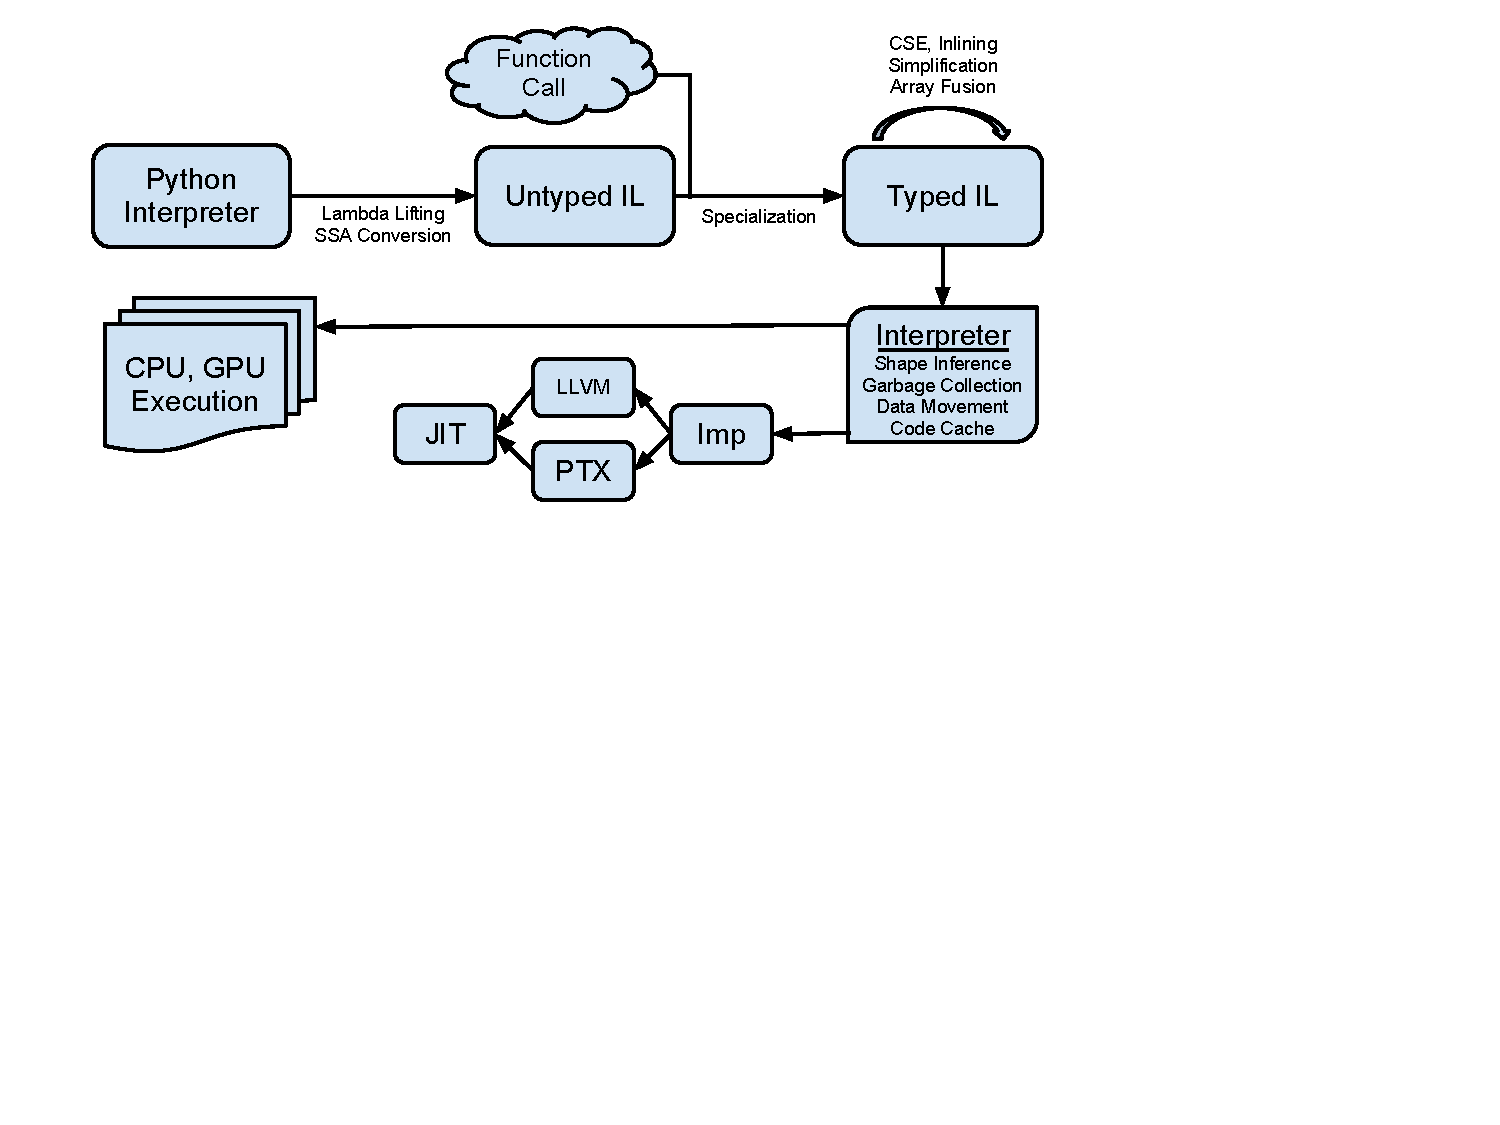
\includegraphics[scale=0.6, trim=0pt 310pt 140pt 80pt]{ParakeetNumPyOverview.pdf}
\end{center}
\caption{Parakeet Pipeline}
\label{fig:overview}
\end{figure*}

\section{Parakeet Runtime and Internals}
We will refer to the following code example (taken from our K-Means clustering benchmark) to help illustrate the process by which Parakeet transforms and executes code. The function \lstinline{minidx} takes as input a matrix \lstinline{C} and a vector \lstinline{x} and then computes the index of the row in \lstinline{C} whose distance from \lstinline{x} is smallest.

\begin{lstlisting}[language=Python,frame=single, label=MinIdx]
def sqr_dist(x,y):
  return sum((x-y) * (x-y))

@PAR
def minidx(C,x):
  sqr_dists = map(sqr_dist,C,fixed=[x])
  return argmin(sqr_dists)
\end{lstlisting}

When the Python interpreter reaches the definition of \lstinline{minidx}, it invokes the \lstinline{@PAR} decorator which translates the syntax tree of \lstinline{minidx} into Parakeet's untyped internal representation.  This internal representation is then converted to Static Single Assignment form \cite{Cytr91}. 

\subsection{Type Specialization}
Parakeet intercepts calls to \lstinline{minidx} and uses the argument types to synthesize a typed version of the function. All functions called by \lstinline{minidx} are also recursively specialized. In our code example, if \lstinline{minidx} were called with a 2D \lstinline{float} array and a 1D \lstinline{float} array then \lstinline{sqr_dist} would be specialized for two 1D \lstinline{float} arrays.

In Parakeet's typed representation, every function must have unambiguous input and output types. To eliminate polymorphism Parakeet inserts casts and $\MAP$ operators where necessary. When \lstinline{sqr_dist} is specialized for vector arguments, its math operators are rewritten into 1D $\MAP$s of those same operators.

The actual process of type specialization is implemented by interleaving an abstract interpreter which propagates input types to infer local types and a rewrite engine which inserts coercions where necessary.

\subsection{Optimization}
In addition to standard compiler optimizations (such as constant folding, function inlining, and common sub-expression elimination), we employ fusion rules~\cite{Jones01} to combine array operators. Fusion enables us increase the computational density of generated code and to avoid the creation of unnecessary array temporaries.

\subsection{Execution}
We have implemented three backends for Parakeet thus far: CPU and GPU backends for JIT compiling native code, as well as an interpreter for handling functions that cannot themselves be parallelized but may contain nested parallelizable operators.

Once a function has been type specialized and optimized, it is handed off to Parakeet's scheduler which is responsibile for choosing among these three backends.  For each array operator, the scheduler employs a simple cost-based heuristic which considers nested array operators, data sizes, and memory transfer costs to decide where to execute it.

Accurate prediction of array shapes is necessary both for the allocation of intermediate values on the GPU as well as for the above cost model determining placement of computations. We employ a simple abstract interpreter which propagates shape information through a function using the obvious shape semantics for each operator. For example, a $\REDUCE$ operation collapses the outermost dimension of its argument whereas a $\MAP$ preserves a shape's outermost dimension.

When the scheduler encounters a nested array operator -- e.g.~a $\MAP$ whose payload function is itself a $\REDUCE$ -- it needs to choose which operator, if any, will be parallelized.  If an array operator is deemed a good candidate for native hardware execution, the function argument to the operator is then inlined into a program skeleton that implements the operator. Parakeet flattens all nested array computations within the function argument into sequential loops.

Several systems similar to Parakeet \cite{Cata11,Chaf11} generate GPU programs by emitting CUDA code which is then compiled by NVIDIA's CUDA nvcc toolchain. Instead, Parakeet emits GPU assembly code directly since the compile times are dramatically shorter. To generate CPU code we use the LLVM compiler framework~\cite{Latt02}.

\section{Evaluation}
\label{Evaluation}

We evaluate Parakeet on two benchmarks: Black-Scholes option pricing, and K-Means Clustering.  We compare Parakeet against hand-tuned CPU and GPU implementations.  Due to space constraints, and since at the time of writing our CPU backend only supports single-threaded execution, we only present GPU results for Parakeet.  For Black-Scholes, the CPU reference implementation is taken from the PARSEC \cite{Bien08} benchmark suite, and the GPU implementation is taken from the CUDA SDK \cite{NvidSD}.  For K-Means Clustering both the CPU and GPU reference versions come from the Rodinia benchmark suite~\cite{Che09}.  For both benchmarks, we ported the reference implementations as directly as possible from their source languages to Parakeet.

We ran all of our benchmarks on a machine running 64-bit Linux with an Intel Core i7 3.2GHz 960 4-core CPU  and 16GB of RAM.  The GPU used in our system was an NVIDIA Tesla C1060 with 240 vector lanes, a clock speed of 1.296 GHz, and 4GB of memory.

\subsection{Black-Scholes}
\label{results-bs}

Black-Scholes option pricing \cite{Blac73} is a standard algorithm used for data parallel benchmarking.  We compare Parakeet against the multithreaded OpenMP CPU implementation from the PARSEC \cite{Bien08} suite with both 1 and 8 threads and the GPU version in the CUDA SDK \cite{NvidSD}.  We modified the benchmarks to all use the input data from the PARSEC implementation so as to have a direct comparison of the computation alone.  We also modified the CUDA version to calculate only one of the call or put price per option so as to match the behavior in PARSEC.

\begin{figure}
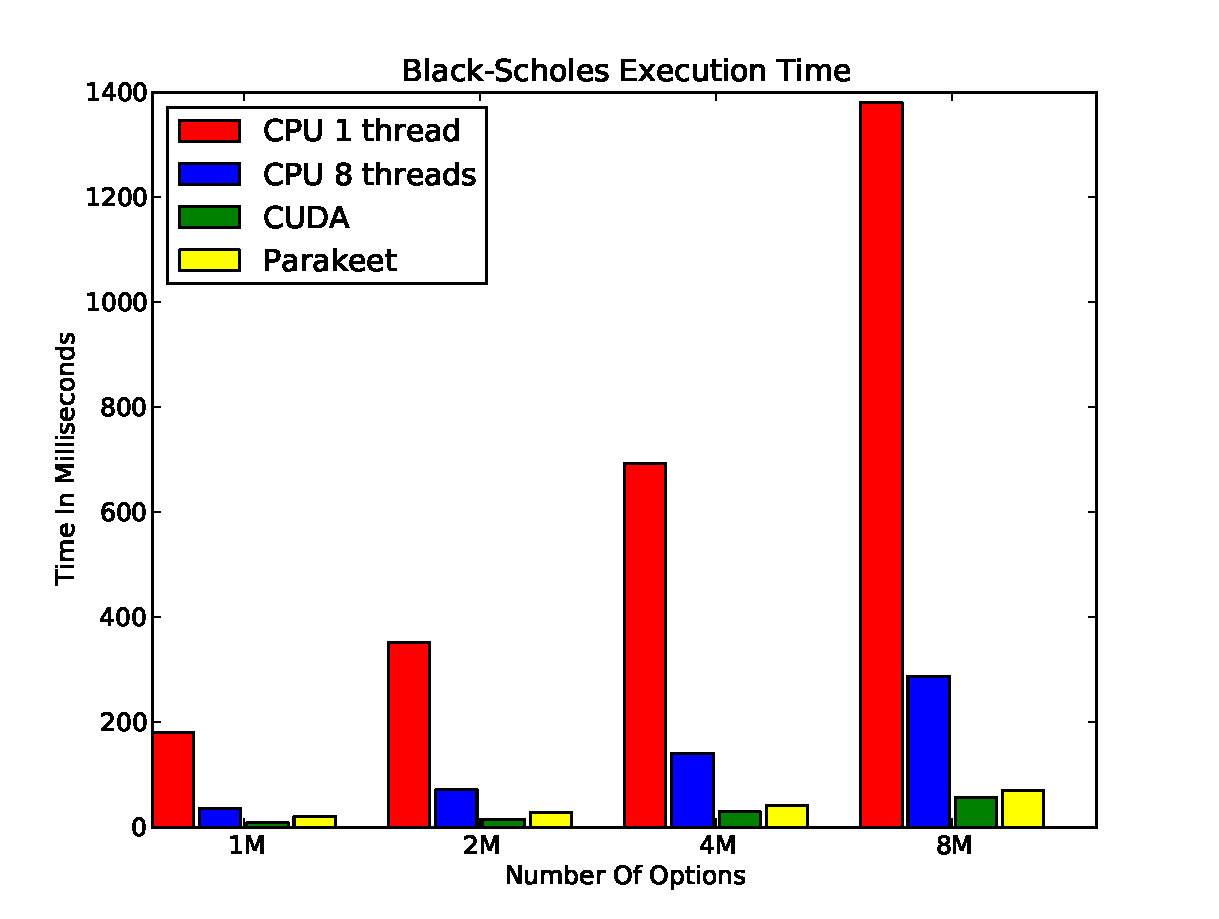
\includegraphics[scale=0.4]{BSWCPU.pdf}
\caption{Black Scholes Total Times}
\label{BSCPU}
\end{figure}

In Figure \ref{BSCPU}, we see the total execution times of the various versions. These times include the time it takes to transfer data to and from the GPU in the GPU benchmarks.  As expected, Black Scholes performs very well on the GPU as compared with the CPU.  We see that Parakeet performs very similarly to the hand-written CUDA version, with overheads decreasing as a percentage of the run time as the data sizes grow since most of them are fixed costs related to dynamic compilation.

\begin{figure}
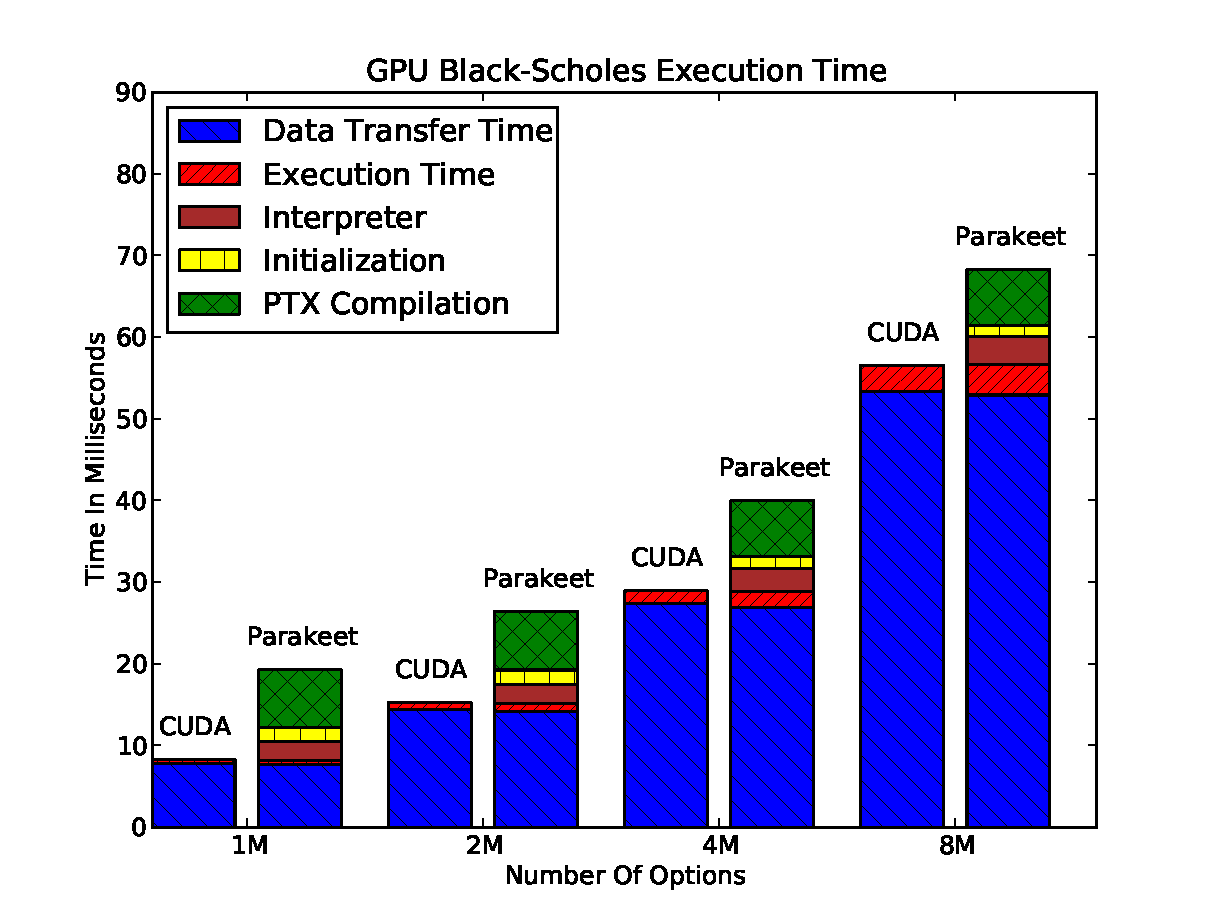
\includegraphics[scale=0.4]{BSNOCPU.pdf}
\caption{Black Scholes GPU Execution Times}
\label{BSGPU}
\end{figure}

In Figure \ref{BSGPU}, we break down Parakeet's performance as compared with the hand-written CUDA version.  The Parakeet run times range from 24\% to 2.4X slower than those of CUDA, with Parakeet performing better as the data size increases.  We can see that transferring data to and from the GPU's memory is expensive and dominates the runtime of this benchmark.  The GPU programs that Parakeet generates are slightly less efficient than those of the CUDA version, with approximately 50\% higher run time on average.  Most of this slowdown is due to compilation overheads.

\subsection{K-Means Clustering}
\label{results-k-means}

\begin{figure}[h!]
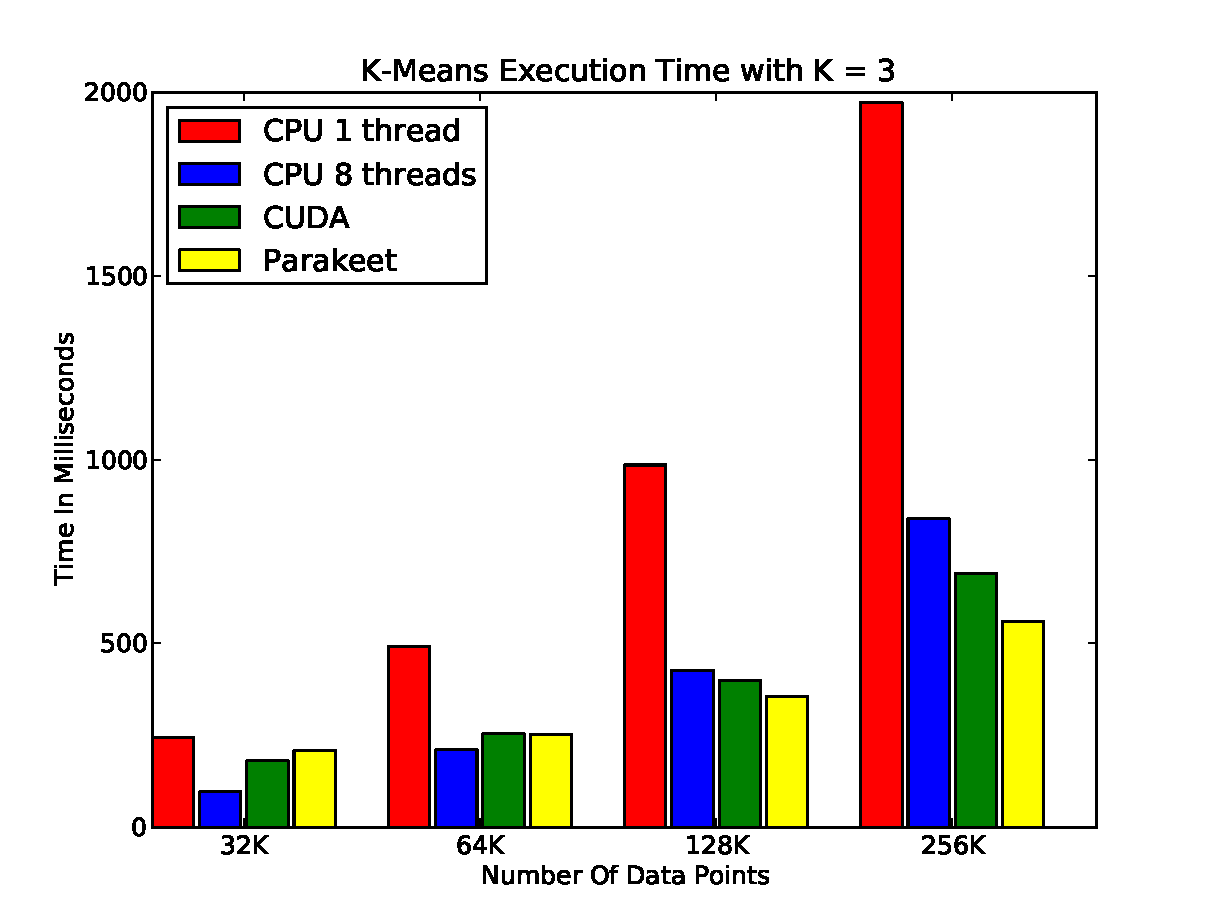
\includegraphics[scale=0.4]{KMCPUK3.pdf}
\caption{K-Means Total Times with 30 Features, K = 3}
\label{KMCPU3}
\end{figure}

We also tested Parakeet on K-Means clustering, a commonly used unsupervised learning algorithm.  We chose K-Means since it includes both loops and nested array operators, and thus illustrates Parakeet's support for both.  The Parakeet code we used to run our benchmarks can be seen in Listing \ref{K-Means-Code}.

In Figure \ref{KMCPU3}, we see the total run times of K-Means for the CPU and GPU versions with K = 3 clusters and 30 features on varying numbers of data points.  Here, the distinction between the GPU and the CPU is far less stark.  In fact, for up to 64K data points the 8-thread CPU version outperforms the GPU.  Further, we see that for more than 64K data points, Parakeet actually performs better than both the CPU and GPU versions.

\begin{figure}[h!]
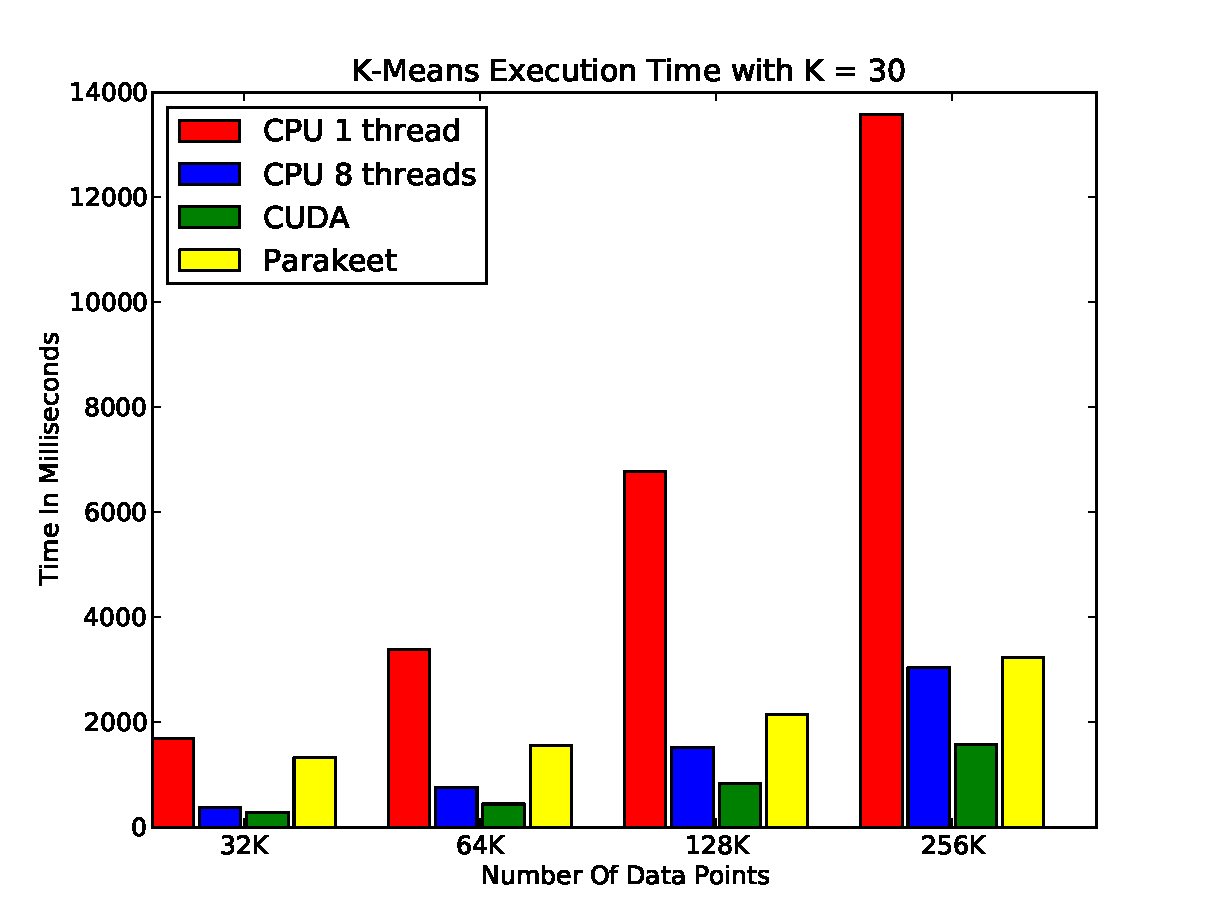
\includegraphics[scale=0.4]{KMCPUK30.pdf}
\caption{K-Means Total Times with 30 Features, K = 30}
\label{KMCPU30}
\end{figure}

The reason Parakeet is able to perform so well with respect to the CUDA version is due to the difference in how they compute the new average centroid for the new clusters in each iteration.  The CUDA version brings the GPU-computed assignment vectors back to the CPU in order to perform this reduction, as it involves many unaligned memory accesses and so has the potential to perform poorly on the GPU.  Parakeet chooses to execute this code on the GPU instead, prefering to avoid the data transfer penalty.  For such a small number of clusters, the Parakeet method ends up performing far better.  However, for larger numbers of clusters (roughly 30 and above), the fixed overhead of launching an individual kernel to average each cluster's points overwhelms the performance advantage of the GPU and Parakeet ends up performing worse than the CUDA version.  We are currently implementing better code placement heuristics based on dynamic information in order to use the GPU only when it would actually be advantageous, in which case Parakeet should perform well for all numbers of clusters.

\begin{lstlisting}[language=Python,frame=single, label=K-Means-Code, caption={K-Means Parakeet Code}]
def calc_centroid(X, a, i):
  return parakeet.avg(X[a == i])

def dist(x, y):
  return numpy.sqrt(
    parakeet.sum((x-y)*(x-y)))

def minidx(C, x):
  return numpy.argmin(
    parakeet.map(dist, C, fixed=[x]))

@PAR
def kmeans(X, k, a):
  C = parakeet.map(calc_centroid,
                   np.arange(k),
                   fixed=[X, a])
  converged = False
  while not converged:
    lastAssignment = a
    a = parakeet.map(minidx, X, fixed=[C])
    C = parakeet.map(calc_centroid,
                     np.arange(k),
                     fixed=[X, a])
    converged = np.all(lastAssignment == a)
  return C
\end{lstlisting}

In Figure \ref{KMCPU30}, we present the run times of K-Means for 30 features and K = 30 clusters.  In this case, the hand-written CUDA version performs best in all cases, though its advantage over the CPU increases and its advantage over Parakeet decreases with increasing data size.  As discussed, the Parakeet implementation suffers from the poorly performing averaging computation that it executes on the GPU, with a best case of an approximate 2X slowdown over the CUDA version.  However, Parakeet exhibits the best scaling of any of the implementations, and would likely close the gap even further at larger data sizes.

\begin{figure}
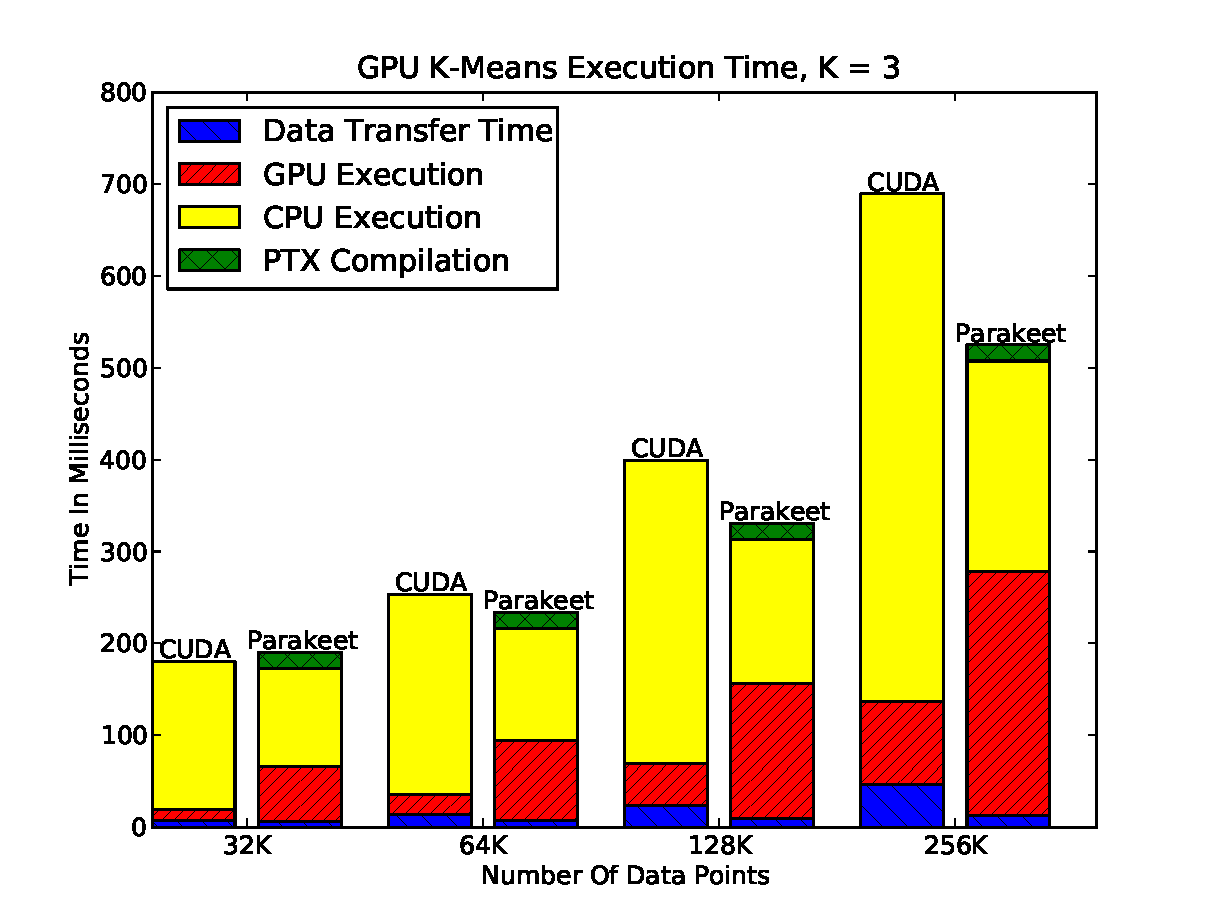
\includegraphics[scale=0.4]{KMGPU.pdf}
\caption{K-Means GPU Times with 30 Features, K = 3}
\label{KMGPU}
\end{figure}

Figure \ref{KMGPU} shows a breakdown of the different factors that contribute to the overall K-Means execution times.  Both Rodinia's CUDA version and Parakeet use the CPU to perform a significant amount of the computation.  The Rodinia version uses the CPU to compute the averages of the new clusters in each iteration, while Parakeet spends much of its CPU time on program analysis and transformation; garbage collection; and setting up GPU kernel launches.  As mentioned above, Parakeet spends much more time on the GPU than the Rodinia version does. In this benchmark, as opposed to Black-Scholes, little of the execution time is spent on data transfers.  It is important to note that the Python implementation of K-Means is orders of magnitude shorter than the CUDA implementation.

\section{Related Work}
\label{RelatedWork}
There have been several projects that use just-in-time compilation to accelerate Python programs on CPUs, but to our knowledge none attempt to generate parallel code.  The PyPy project is an alternative implementation of Python that uses a meta-tracing JIT to achieve an average 5.3X speedup across 20 benchmarks~\cite{Rigo06}. Psyco was a previous Python JIT compiler that achieved significant speedups~\cite{Rigo04}.  A number of recent projects enable the use of embedded DSLs in productivity languages for various tasks, e.g.~ASP~\cite{Cook11} and OptiML~\cite{Chaf11}.

The use of graphics hardware for non-graphical computation has a long history~\cite{Leng90}. The Brook language extended C with ``kernels'' and ``streams'', exposing a programming model similar to what is now found in CUDA and OpenCL~\cite{Buck04}.  Microsoft's Accelerator~\cite{Tard06} was the first project to use high level (collection-oriented) language constructs as a basis for GPU execution. Accelerator's programming model does not support function abstractions (only expression trees) and its only underlying parallelism construct is limited to the production of $\MAP$-like kernels.  Nikola~\cite{Main10} and Accelerate~\cite{Chak11} are first-order array-oriented languages embedded in Haskell. Neither is as convenient to use or as feature rich as Parakeet, either requiring the programmer to manually coordinate computations which require multiple GPU kernel launches or lacking support for nested array operators.

Copperhead parallelizes a statically typed, purely functional array subset of Python through the dynamic compilation and execution of CUDA kernels~\cite{Cata11}. Copperhead supports nested array computations, and has a notion of scheduling computation on both GPUs and CPUs (although no CPU backend has been implemented). Unlike Parakeet, Copperhead does not use dynamic information when making scheduling decisions and thus must rely on user annotations. Copperhead's array operators are implemented by C++ templates. Targeting C++ allows easy integration of the Thrust GPGPU library~\cite{Hobe10} but incurs long compilation times. Copperhead disallows polymorphism: neither implicit scalar casts nor NumPy-style array broadcasting are possible within its type system. By contrast, since Parakeet's more flexible type specializer translates polymorphism into coercions it is able to execute code that uses NumPy constructs. This allows Parakeet to accelerate NumPy programs with minimal changes.

\section{Conclusion}
\label{Conclusion}
Parakeet allows the programmer to write Python code using a widely-used numerical computing library while achieving good performance on modern parallel hardware. Parakeet automatically synthesizes and executes efficient native binaries from Python code. Parakeet is a usable system in which complex programs can be written and executed efficiently.  On two benchmark programs, Parakeet delivers performance very competitive with even hand-tuned GPU implementations.  Parakeet code can coexist with standard Python code, allowing full interoperability with all of Python's tools and libraries.

In the near future, we plan to add support for generating multithreaded CPU programs to our CPU backend and add support for splitting work simultaneously across CPUs and GPUs.

{\small
\bibliographystyle{acm}
\bibliography{../Parallelism}{}
}
\end{document}
